
\subsection{Tab}
I det følgende afsnit estimeres tabet i MOSFET, diode og transformator. Derudover beregnes det samlede tab, og dermed også effektiviteten, i converteren. Tabene i komponenterne estimeres ved, at måle temperaturstigningen og derudfra regne tabet ud fra den termiske modstand i kølepladen og kerneformen.

Først estimeres tabet i MOSFET'en. Figur~\ref{fig:temp_mosfet} viser temperaturmålingen af denne. Her måles temperaturen til $72.8\degreeCelsius$, som giver temperaturstigning på $72.8\degreeCelsius - 25\degreeCelsius = 47.8\degreeCelsius$. Den brugte køleplade har en termisk modstand på $9.5K/W$\cite{Heatsink}. Ud fra dette kan effektafsættelsen i MOSFET'en regnes.

\begin{equation}
P_{MOSFET} = \frac{47.8\degreeCelsius}{9.5K/W} = 5.03W
\end{equation}



\begin{figure}[H]
	\center
	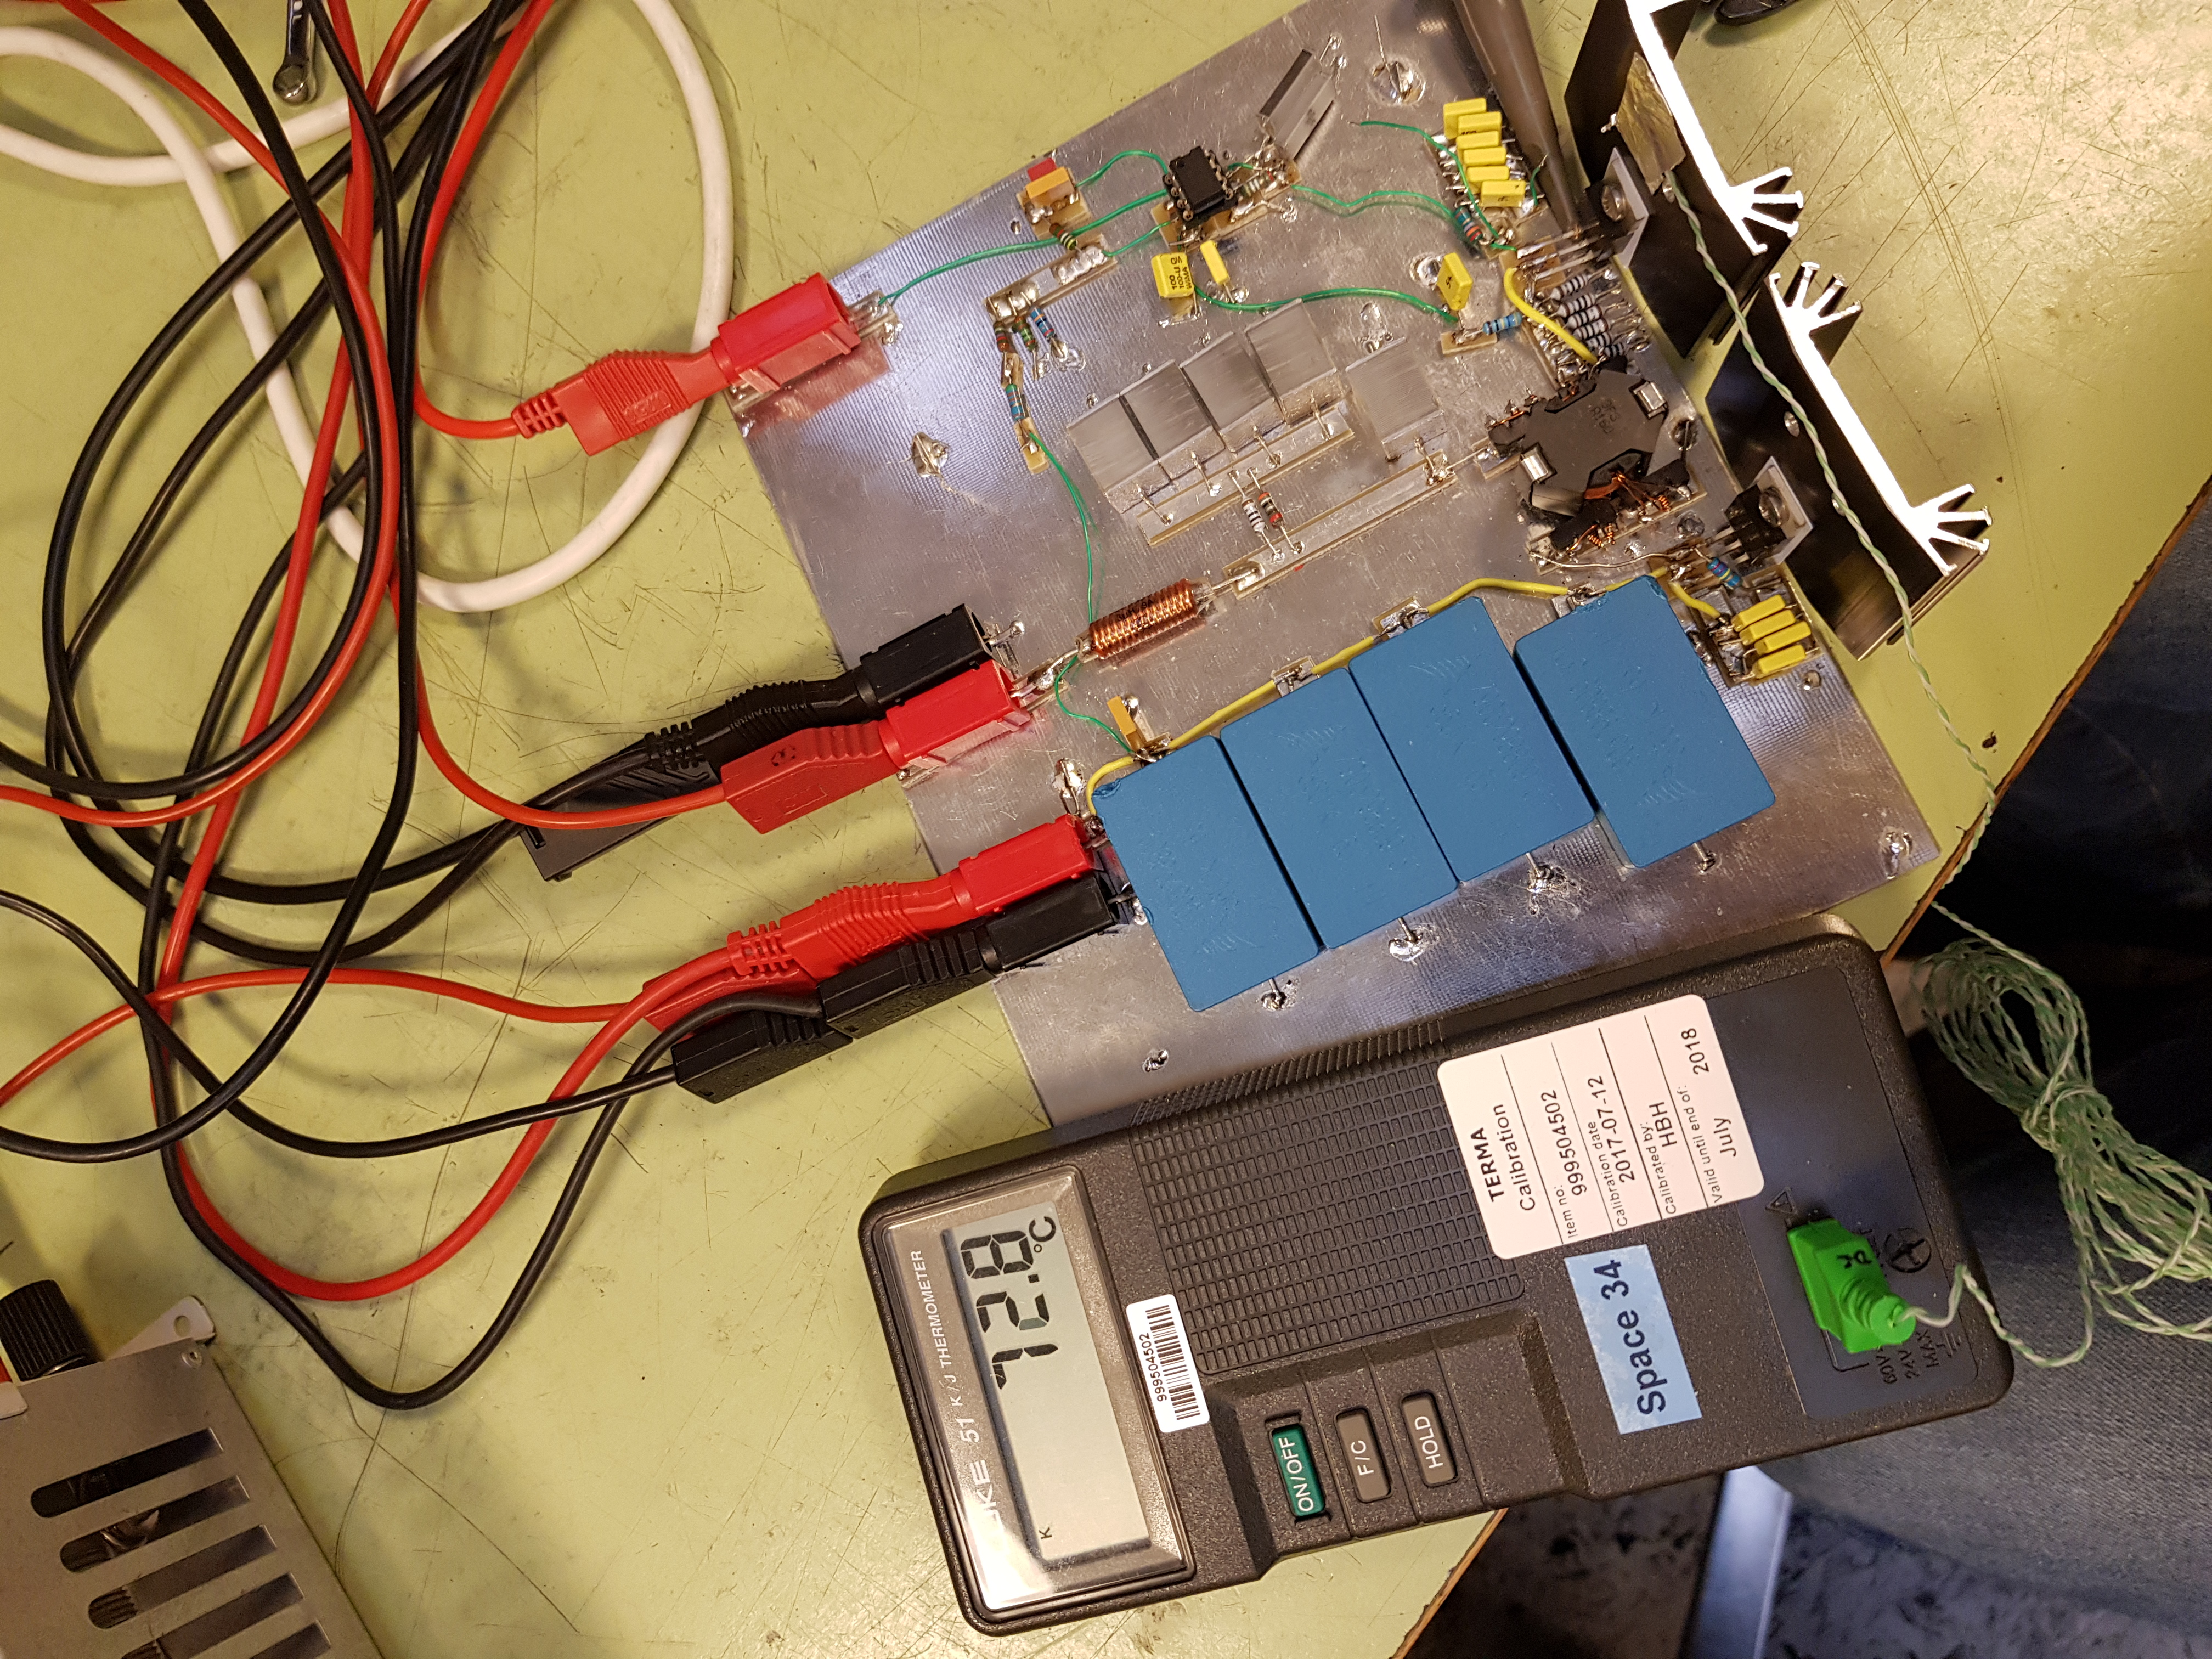
\includegraphics[max width=0.7\linewidth, angle=-90]{/tex/2iteration/billeder/Realisering/MOSFET.jpg}
	\caption{Temperaturmåling MOSFET}
	\label{fig:temp_mosfet}
\end{figure}

Nu måles temperaturstigningen i dioden. Her bruges samme køleplade, og derfor også samme termiske modstand. På figur~\ref{fig:temp_diode} aflæses temperaturen i dioden til $41.8\degreeCelsius$, det giver en temperaturstigning på $41.8\degreeCelsius - 25\degreeCelsius = 16.8\degreeCelsius$. Ud fra dette kan effektafsættelsen i dioden regnes. I analysen blev dette regnet til $1.13W$. Afvigelsen kan tyde på, at moduleringen af tabet i dioden ikke er præcist nok, eller spændingsfaldet over dioden er større end forventet.

\begin{equation}
P_{diode} = \frac{16.8\degreeCelsius}{9.5K/W} = 1.77W
\end{equation}

\begin{figure}[H]
	\center
	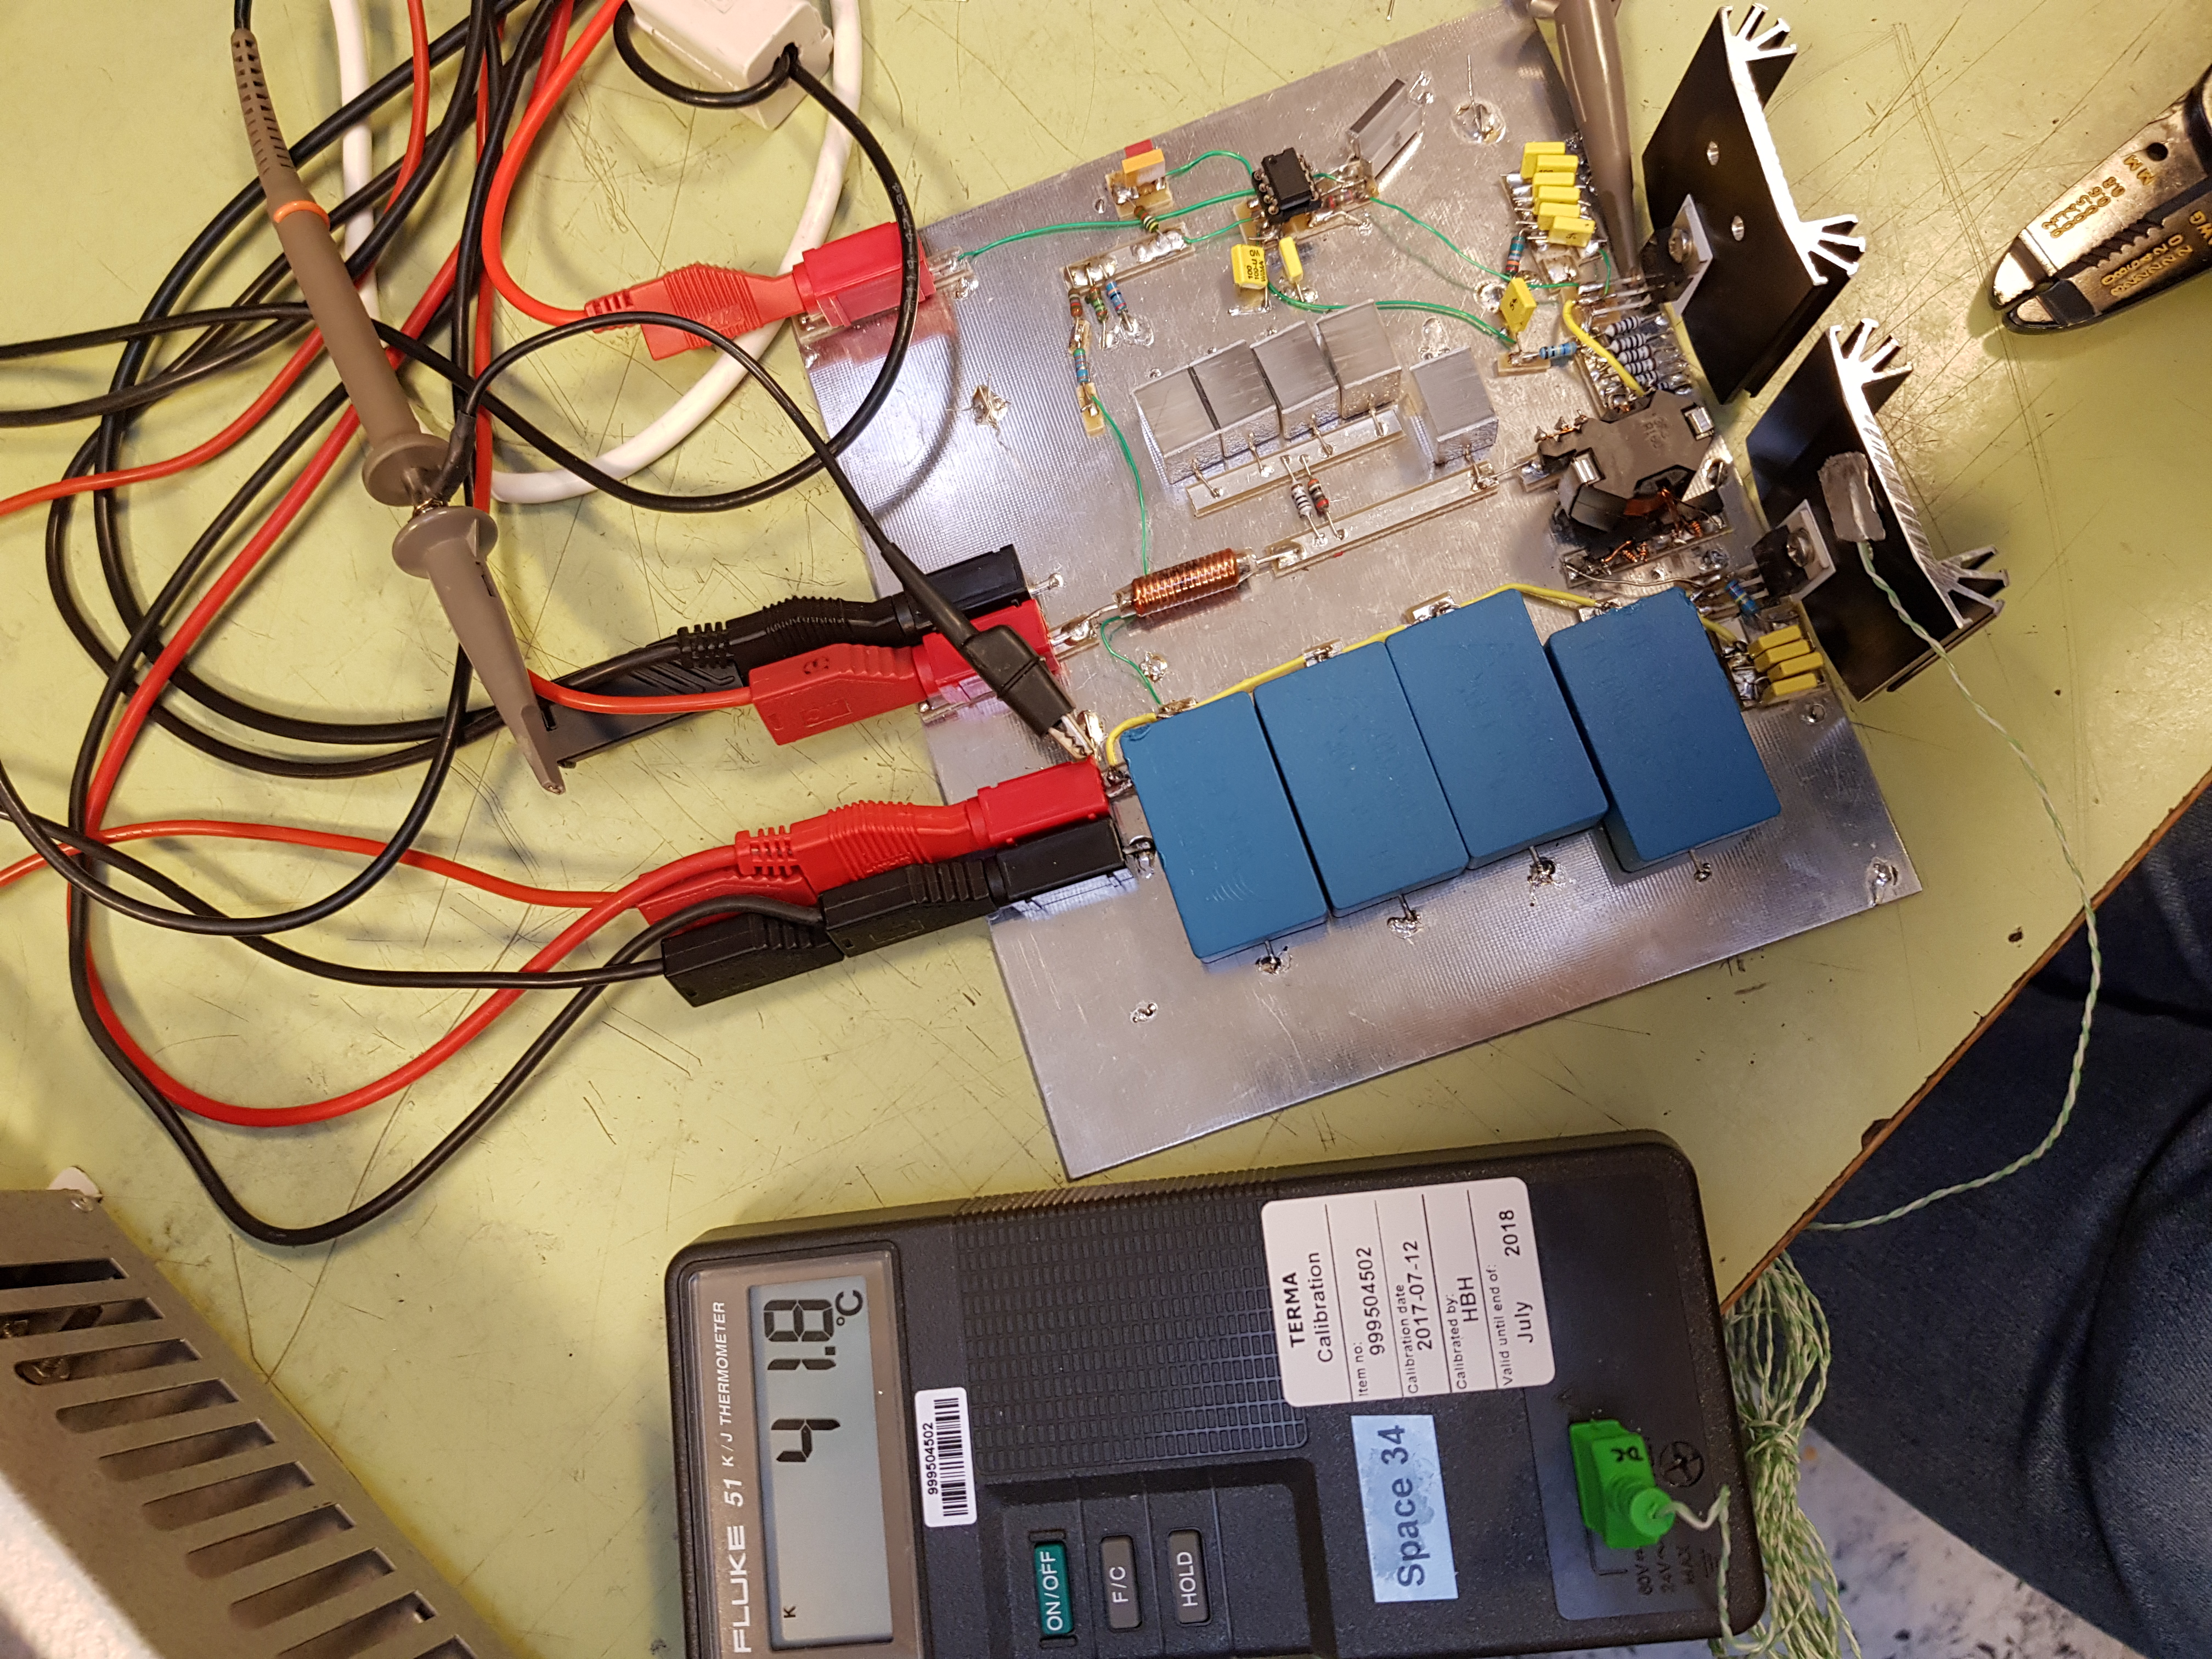
\includegraphics[max width=0.7\linewidth, angle=-90]{/tex/2iteration/billeder/Realisering/Diode.jpg}
	\caption{Temperaturmåling diode}
	\label{fig:temp_diode}
\end{figure}

Til sidst måles temperaturen i transformatoren. Dette er gjort på figur~\ref{fig:temp_trans}, hvor temperaturen aflæses til $70.6\degreeCelsius$ hvilket giver en temperaturstigning på $70.6\degreeCelsius - 25\degreeCelsius = 45.6\degreeCelsius$. Den termiske modstand i kerne formen aflæses i et datablad for en RM8 kerne til $57K/W$\cite{epcos-cores}. Ud fra dette kan effektafsættelsen i transformatoren regnes.

\begin{equation}
P_{trans} = \frac{45.6\degreeCelsius}{57K/W} = 0.8W
\end{equation}

\begin{figure}[H]
	\center
	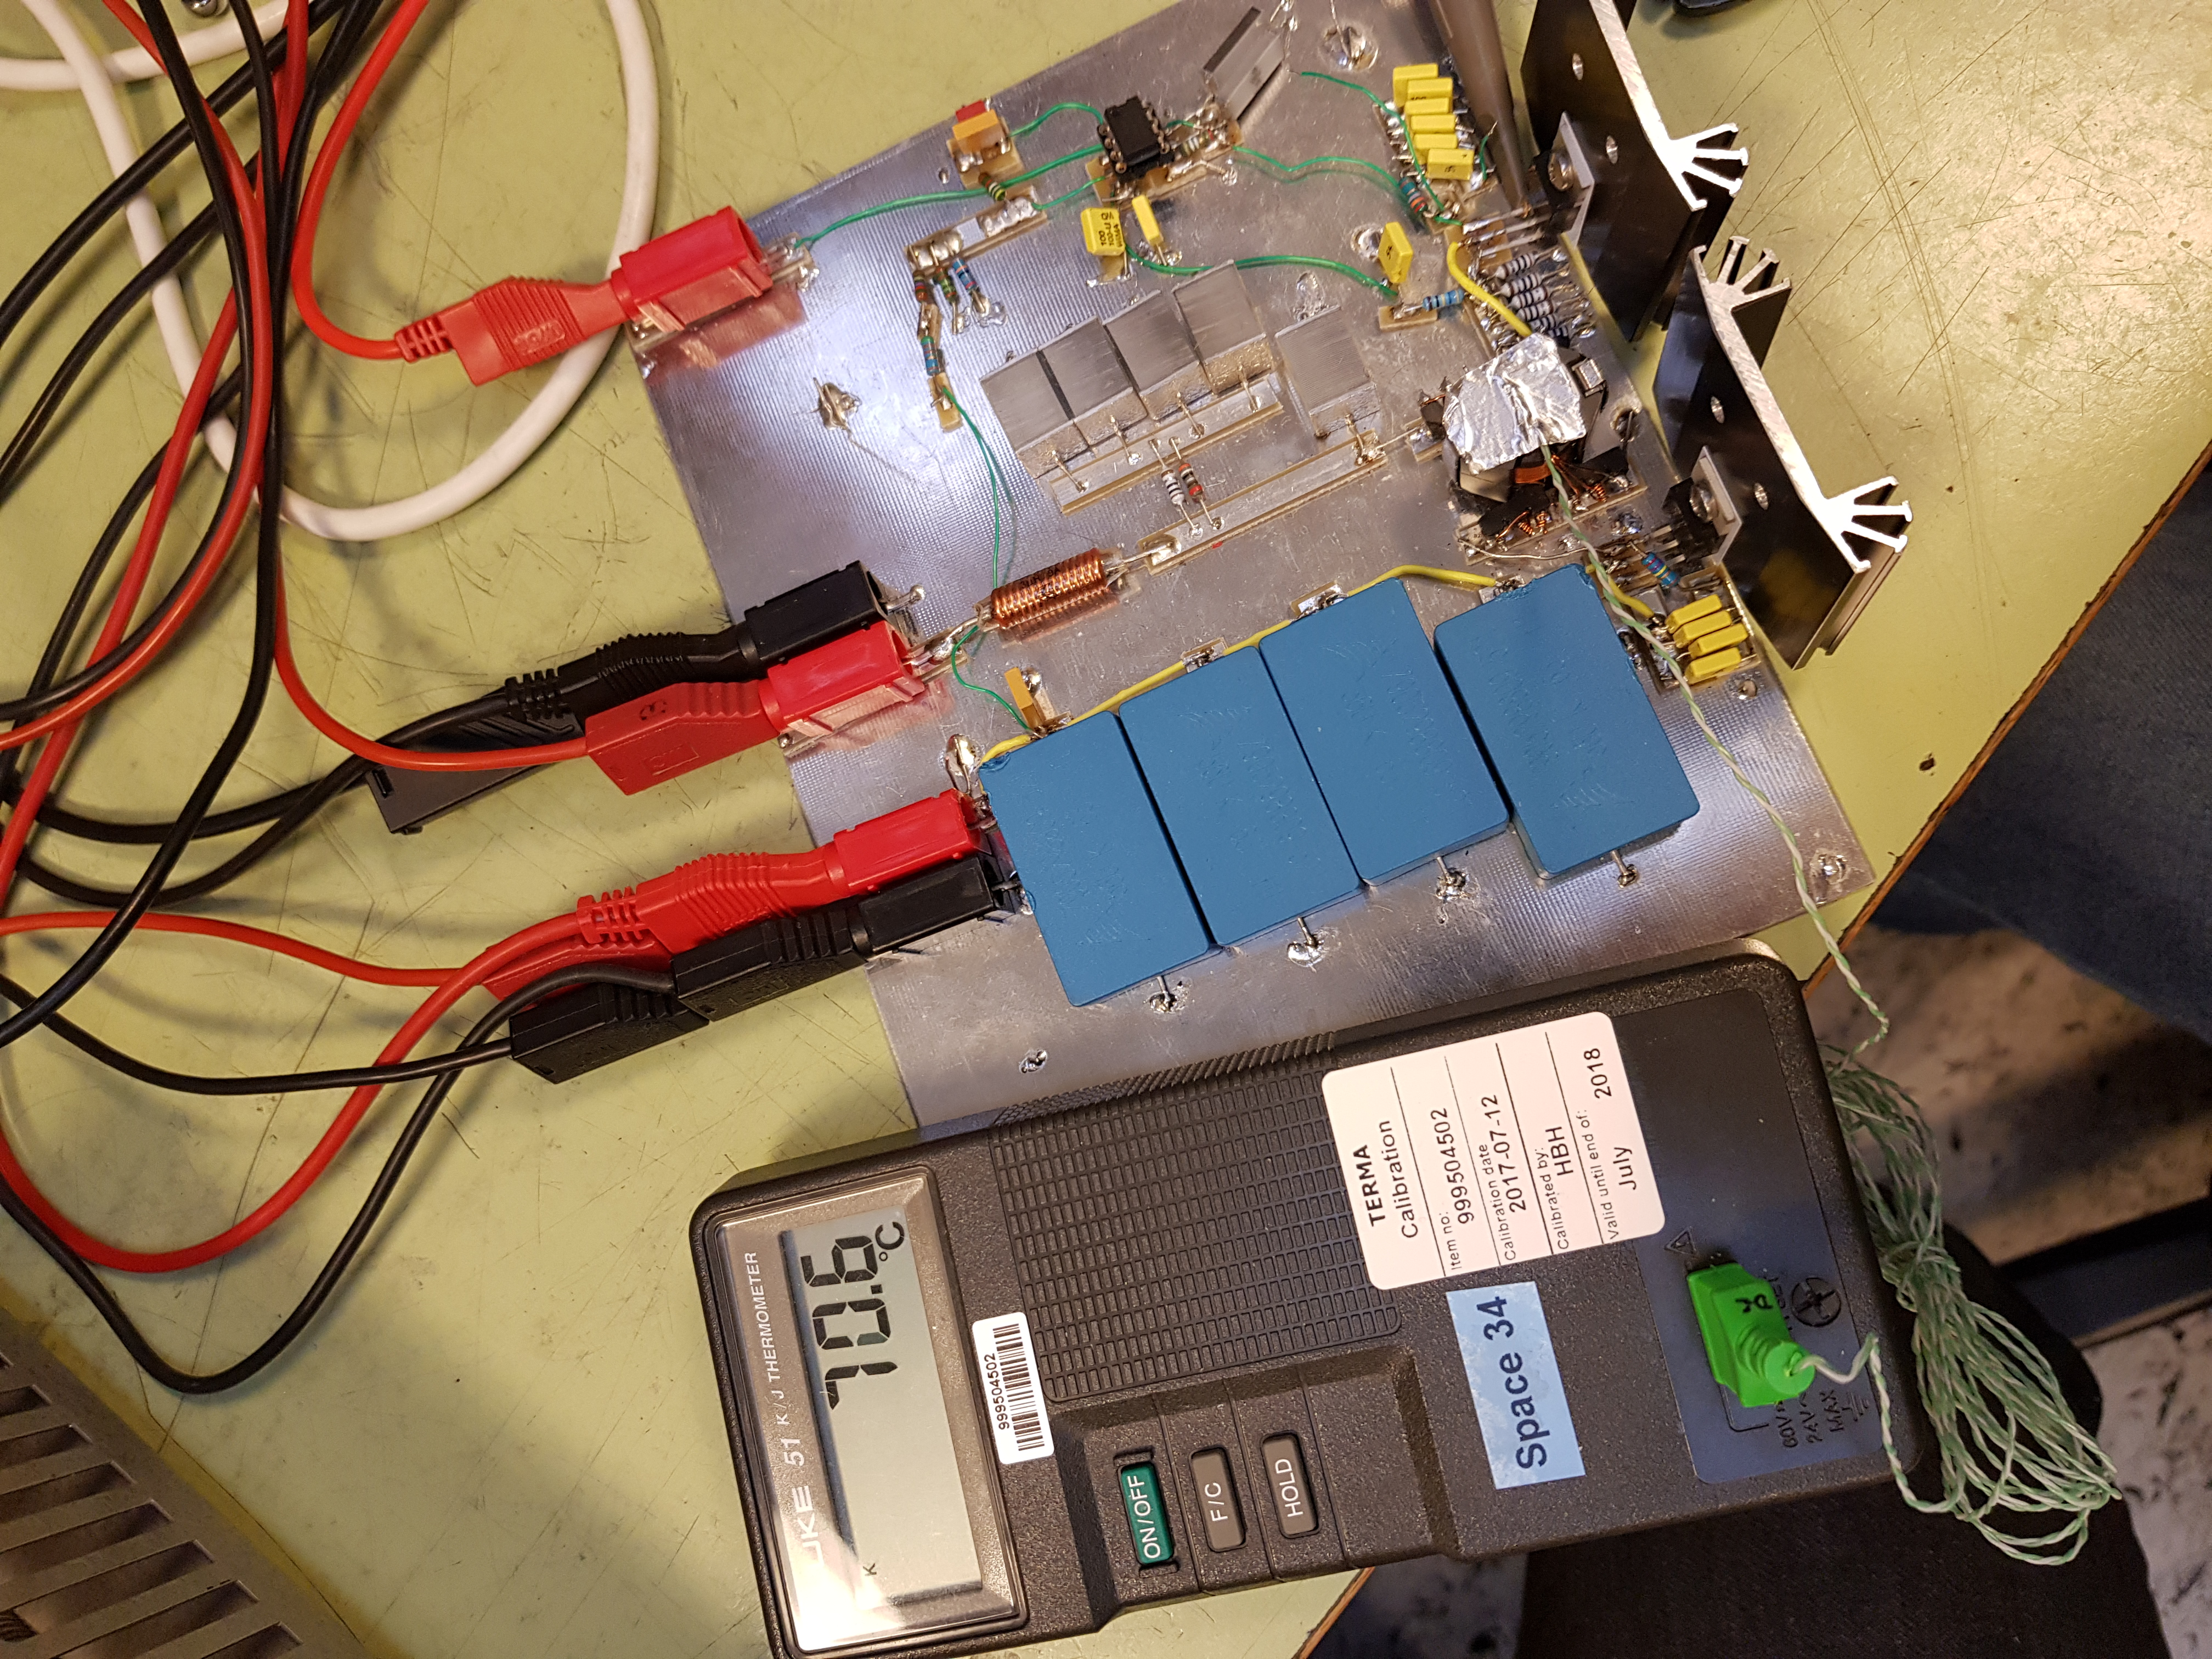
\includegraphics[max width=0.7\linewidth, angle=-90]{/tex/2iteration/billeder/Realisering/Transformator.jpg}
	\caption{Temperaturmåling transformator}
	\label{fig:temp_trans}
\end{figure}

Converterens effektivitet regnes ved forholdet mellem udgangseffekten og indgangseffekten. Disse findes ved, at måle strømme og spændinger på indgang og udgang. Indgangseffekten, udgangseffekt og effekttab regnes ved følgende ligninger.

\begin{equation}
P_{in} = V_{in} \cdot I_{in} = 26V \cdot 2.35A = 61.1W
\end{equation}

\begin{equation}
P_{out} = V_{out} \cdot I_{out} = 21.07V \cdot 2.49A = 52.5W
\end{equation}

\begin{equation}
P_{loss} = P_{in} - P_{out} = 61.1W - 52.5W = 8.6W
\end{equation}

\noindent Ud fra indgangs- og udgangseffekten regnes også den endelige effektivitet i converteren. 

\begin{equation}
\eta = \frac{P_{out}}{P_{in}} \cdot 100 = \frac{52.5W}{61.1W} \cdot 100 = 85.87\percent
\end{equation}

Resultaterne indsættes i tabel~\ref{tab:realisering_tab}, sammen med de analyserede og simulerede tab. Her er tabet i current-sense modstandene ikke målt.
\begin{table}[H] 			
	\centering
	\begin{tabularx}{\textwidth}{|X|l|l|l|}
		\hline
		\textbf{\large Komponent} & \multicolumn{3}{|l|}{\textbf{\large Tab}} \\ \hline
		& A & S	& R\\ \hline
		\textbf{Transformator samlet} & $1.46\watt$ & $1.62\watt$ & $0.8\watt$\\ \hline 
		Kernetab & $366m\watt$ & $311m\watt$ &  \\ \hline
		Kobbertab & $1.09\watt$ & $1.31\watt$ & \\ \hline
		& &	& \\ \hline
		\textbf{MOSFET samlet} & $5.55\watt$ & $4.45\watt$ & $5.03\watt$\\ \hline
		Conductiontab & $1.06\watt$ & & \\ \hline
		Switchtab & $4.49\watt$ &  &    \\ \hline
		& &	& \\ \hline
		\textbf{Diode} & $1.13\watt$ & $1.47\watt$ & $1.77\watt$\\ \hline
		& &	& \\ \hline
		\textbf{CS modstands tab} & $1.52\watt$ & $2.03\watt$ & \\ \hline
		& &	& \\ \hline
		\textbf{Total tab} & $9.67\watt$ & $9.57\watt$ & $8.6\watt$\\ \hline
	\end{tabularx}
	\caption{Oversigt over analyseret, simuleret og realiseret tab}
	\label{tab:realisering_tab}
\end{table}




